\documentclass[final]{beamer}

\usepackage[utf8]{inputenc}
\usepackage[frenchb]{babel}
\usepackage{verbatim}
\usepackage{graphicx}
\usepackage{color}
\usepackage{hyperref}
\usepackage{verbatim}
\usepackage{url}

\usepackage{pifont}
\newcommand{\cmark}{\ding{51}}%
\newcommand{\xmark}{\ding{55}}%

\usepackage{multirow}

\hypersetup{colorlinks=true, linkcolor=black, urlcolor=blue}
\beamertemplatenavigationsymbolsempty
\setbeamertemplate{sections/subsections in toc}[circle]

\selectcolormodel{cmyk}

\definecolor{i6blue}{cmyk}{1,0.305,0,0.06}
\definecolor{i6bluedark}{rgb}{0.0156,0.2578,0.5625}
\definecolor{i6colorscheme1}{HTML}{FFFFFF}  % e.g. for block title
\definecolor{i6colorblockbg}{HTML}{ADDFFF}
\definecolor{i6colorblockfg}{HTML}{FFFFFF}
\definecolor{i6colorscheme2}{HTML}{100D09}  % e.g. title in headline
\definecolor{i6colorscheme3}{HTML}{FFFFFF}  % e.g. for poster background
\definecolor{i6colorscheme4}{HTML}{000000}
\definecolor{i6colorschemeHeadline}{HTML}{FFFFFF}  % for headline bg
\definecolor{i6colorschemeFootline}{HTML}{100D09}  % for headline bg

\setbeamercolor{headline}{fg=blue,bg=i6colorschemeHeadline}
\setbeamercolor{title in headline}{fg=blue}
\setbeamercolor{author in headline}{fg=black}
\setbeamercolor{institute in headline}{fg=lightgray}
\setbeamercolor{logo in headline}{fg=black,bg=lightgray}
\setbeamercolor{separation line}{bg=i6colorscheme1}

\definecolor{lightgreen}{rgb}{0.0,0.8,0.0}
\definecolor{lightblue}{rgb}{0.3,0.8,1.0}
\definecolor{lightred}{rgb}{0.874,0.180,0.105}
\definecolor{gray}{rgb}{0.4,0.4,0.4}
\definecolor{lightgray}{rgb}{0.8,0.8,0.8}
\definecolor{shadecolor}{rgb}{0.9,0.9,0.9}

\usepackage{multirow}

\title{Simple connectome inference from partial\\[1ex]
correlation statistics in calcium imaging}
\author{{\small Antonio Sutera, Arnaud Joly, Vincent François-Lavet, Zixiao Aaron Qiu\\[1ex] Gilles Louppe, Damien Ersnt and Pierre Geurts.}}
\date{}



\begin{document}

%% Slide 1 ==================================================================

\begin{frame}
	
\vspace{-0cm}

	\begin{center}
	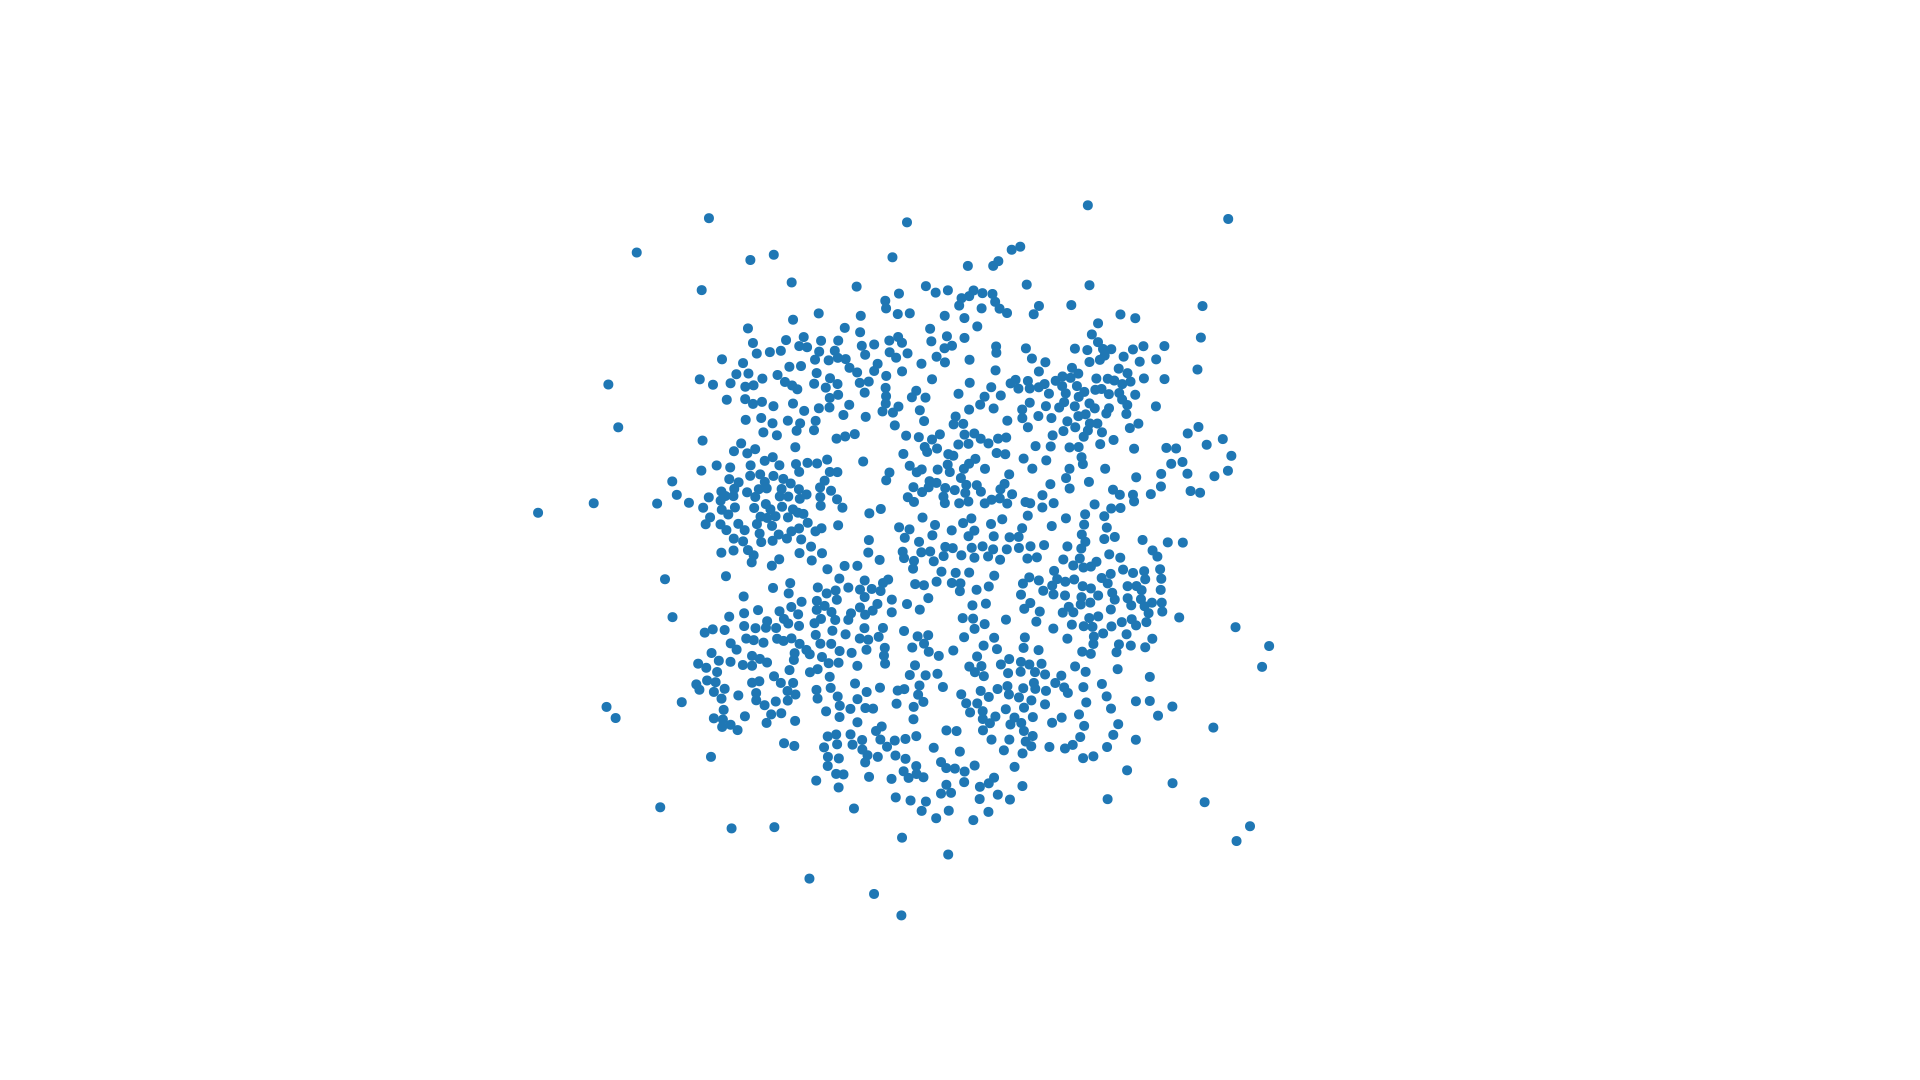
\includegraphics[width=7cm]{images/network.png}
	\end{center}

\vspace{-9.5cm}
  \begin{beamercolorbox}[wd=\paperwidth, ignorebg]{headline}
    \begin{center}
      
      \usebeamercolor{title in headline}{\color{fg}\Large{\textbf{\inserttitle}}\\[2ex]}
      \usebeamercolor{author in headline}{\color{fg}\small{\insertauthor}\\[1ex]}
    \end{center}
  \end{beamercolorbox}

\end{frame}


%% Slide 2 ==================================================================

\begin{frame}

\frametitle{Introduction}


From {\color{i6blue} time-series of the neuron activity}, the \textbf{goal} is to {\color{red} \textbf{infer} the directed connections between neurons}.

\end{frame}

%% Slide 3 ==================================================================

\begin{frame}

\frametitle{Introduction}


But this problem is \textbf{difficult} because of...


\begin{tabular*}{\textwidth}{l r} \hline
&\multirow{3}{*}{\includegraphics[width=2cm]{images/miss.png} \includegraphics[width=2cm]{images/hidden.png}}\\ 

{\color{red} \textbf{masking} effects}
& \\ 
& \\
\end{tabular}

% \begin{itemize}
% \item {\color{red} \textbf{masking} effects},
% \includegraphics[width=2cm]{images/miss.png} \includegraphics[width=2cm]{images/hidden.png}
% \item {\color{red} \textbf{low} sampling rate},
% \includegraphics[width=4cm]{images/slowsamplingrate.png}
% \item {\color{red} \textbf{slow} decay} of fluorescence.
% \includegraphics[width=4cm]{images/original_curve_gr}
% \end{itemize}

\end{frame}

%% Slide 4 ==================================================================

\begin{frame}

\frametitle{Framework of our solution  \hspace{15pt} {\small Table of contents} }

{\color{red} How-to}:
\begin{enumerate}
\item \textbf{Deal} with calcium fluorescence signals: {\color{i6blue} signal processing}.
\item \textbf{Find} the network: the {\color{i6blue} {inference} method}.
\item \textbf{Improve} the method: our {\color{i6blue} {tricks}}.
\end{enumerate}\vskip5pt

{\color{red} One step further}:
\begin{itemize}
\item Improvement of each stage of our solution.
\item Comparison with other methods.
\end{itemize}\vskip5pt

{\color{red} Even further}: 
\begin{itemize}
\item The ``full method'' in a nutshell.
\end{itemize}

\end{frame}

%% Slide 5 ==================================================================

\begin{frame}

\frametitle{Signal processing}

\begin{overprint}
\onslide<1> 
a-b

\onslide<2>
a-b-c

\onslide<3>
a-b-c-d

\onslide<4>
a-b-c-d-e
\end{overprint}

\end{frame}

%% Slide 6 ==================================================================

\begin{frame}

\frametitle{Connectome \textbf{inference} from {\color{red} partial correlation statistics}}

\begin{columns}
\begin{column}{0.5\linewidth}
diag
\end{column}
\begin{column}{0.5\linewidth}

\begin{itemize}
\item[{\color{green} \cmark}] Only direct associations
\item[{\color{green} \cmark}] Filter out spurious indirect effects
\item[{\color{green} \cmark}] Symmetric \\[5ex]
\item[{\color{red} \xmark}] Edge orientation
\item[{\color{red} \xmark}] Sensitive to the value of parameters in the filtering process
\end{itemize}

\end{column}

\end{columns}

\end{frame}

%% Slide 7 ==================================================================

\begin{frame}
\frametitle{Improvements}

\begin{itemize}
\item \textcolor{red}{\textbf{Approximation}} for partial correlation statistics using only the \textcolor{i6blue}{800 first principal components}. \\[5ex]
\item {\color{red} \textbf{Averaged} partial correlation statistics} over various values of the parameters
	\begin{itemize}
		\item[{\color{green} \cmark}] Improve robustness (over all networks)
		\item[{\color{green} \cmark}] Reduce variance of its prediction
		\item[{\color{green} \cmark}] Decrease the sensitivity to the filtering process
	\end{itemize}
\end{itemize}

\end{frame}

%% Slide 8 ==================================================================

\begin{frame}
\frametitle{Each stage of our solution is good!}


\begin{table}[t]
\caption{Performance on \textit{normal-1,2,3,4} with partial correlation and different filtering functions.}
\label{tab:comparison}
\centering
\tiny
\begin{tabular}{| l | c c c c | c c c c |}
\hline
& \multicolumn{4}{c|}{AUROC} & \multicolumn{4}{c|}{AUPRC} \\
\textit{Method} $\backslash$ \textit{normal-} & \textit{1} & \textit{2} & \textit{3} & \textit{4} & \textit{1} & \textit{2} & \textit{3} & \textit{4} \\
\hline
\hline
No  filtering       					& 0.777 & 0.767 & 0.772 & 0.774 & 0.070 & 0.064 & 0.068 & 0.072\\
$ h \circ g \circ f_1$                  & 0.923 & 0.925 & 0.923 & 0.922 & 0.311 & 0.315 & 0.313 & 0.304\\
$ w \circ h \circ g \circ f_1$          & 0.931 & 0.929 & 0.928 & 0.926 & 0.326 & 0.323 & 0.319 & 0.303\\
+ PCA         							& 0.932 & 0.930 & 0.928 & 0.926 & 0.355 & 0.353 & 0.350 & 0.333\\
Averaging           					& 0.937 & 0.935 & 0.935 & 0.931 & 0.391 &  0.390 &  0.385 & 0.375\\
Full method           					& \textbf{0.943} & \textbf{0.942} & \textbf{0.942} & \textbf{0.939} & \textbf{0.403} & \textbf{0.404} & \textbf{0.398} & \textbf{0.388}\\
\hline
\end{tabular}
\end{table}



\end{frame}

%% Slide 9 ==================================================================

\begin{frame}
\frametitle{Comparison with other methods}



\begin{table}[t]

\caption{Performance on \textit{normal-1,2,3,4} with different methods.}
\label{tab:comparison}
\centering
\tiny
\begin{tabular}{| l | c c c c | c c c c |}
\hline
& \multicolumn{4}{c|}{AUROC} & \multicolumn{4}{c|}{AUPRC} \\
\textit{Method} $\backslash$ \textit{normal-} & \textit{1} & \textit{2} & \textit{3} & \textit{4} & \textit{1} & \textit{2} & \textit{3} & \textit{4} \\
\hline
\hline
Averaging           					& 0.937 & 0.935 & 0.935 & 0.931 & 0.391 &  0.390 &  0.385 & 0.375\\
Full method           					& \textbf{0.943} & \textbf{0.942} & \textbf{0.942} & \textbf{0.939} & \textbf{0.403} & \textbf{0.404} & \textbf{0.398} & \textbf{0.388}\\
\hline
PC & 0.886 & 0.884 & 0.891 &  0.877 & 0.153 & 0.145 & 0.170 & 0.132\\
GTE & 0.890 & 0.893 & 0.894 & 0.873 & 0.171 & 0.174 & 0.197 & 0.142\\
GENIE3 & 0.892 & 0.891 & 0.887 & 0.887 & 0.232 & 0.221 & 0.237 & 0.215 \\
\hline
\end{tabular}
\end{table}

\end{frame}


%% Slide 10 =================================================================

\begin{frame}
\frametitle{An optimized version to win the challenge: ``Full method''}

\begin{itemize}
\item A \textbf{tuned} signal processing,
\item \textbf{Weighted} average of partial correlation statistics,
\item \textbf{Prediction} of edge orientation.
\end{itemize}

\end{frame}

%% Slide 11 =================================================================

\begin{frame}
\frametitle{For every details of our method...}

\textbf{The description of the method:}
\begin{itemize}
\item[] Sutera, A., Joly, A., François-Lavet, V., Qiu, Z. A., Louppe, G., Ernst, D., \& Geurts, P. (2014). Simple connectome inference from partial correlation statistics in calcium imaging.\\[7ex]
\end{itemize} 

\textbf{Code available at:}
\begin{itemize}
\item[] \url{https://github.com/asutera/kaggle-connectomics}
\end{itemize}

\end{frame}

\end{document}